\documentclass{acm_proc_article-sp} 
\usepackage{cite}
\usepackage{graphicx}
\begin{document}

\title{Voronoi Treemaps in D3}

\numberofauthors{2} \author{ \alignauthor Peter Henry
  \affaddr{University of Washington}\\ \email{phenry@gmail.com}
  \alignauthor Paul Vines \affaddr{University of
    Washington}\\ \email{paul.l.vines@gmail.com} } \date{21 March
  2014}

\maketitle
\begin{abstract}
Blah blah blah
\end{abstract}


\section{Introduction}
Treemaps are a category of visualizations used for displaying
hierarchical data. While node-and-edge diagrams are often used for
visualizing hierachical structures, treemaps offer some significant
advantages. Primarily, treemaps are space-filling, and therefore allow
each node in a hierarchy to have more viewing area devoted to it than
in a node-and-edge diagram. This allows both larger hierarchies to be
visualized, as well as more detail to be shown on each node, such as
additional text, colors, or glyphs to show attributes of the node.

The majority of treemap layouts used are variants of rectangular
treemaps. These Have the advantage of being relatively fast to layout
and in cases of limited scale produce reasonably understandable
treemaps. However, there are three drawbacks to rectangular treemaps.

First, as hierarchies become deeper, the treemap cells can become
increasingly extreme in aspect ratio, resulting in narrow rectangles
more difficult to see than if their area was distributed in a more
square-like space. This problem is mostly mitigated by various tweaks
to the treemapping algorithm to try to keep the aspect ratio of
regions close to one.

Second, the borders between different regions in the hiearchy can
become difficult to see. In particular, two cells neighboring one
another in the treemap but not siblings in the hierarchy can appear to
share a common edge delineating the same inner node is their parent,
when this is in fact not the case.  Finally, rectangular treemap
algorithms naturally only fill rectangular regions which could be
undesirable for aesthetic or practical reasons.

Voronoi treemaps eliminate these problems. Firstly, Voronoi treemap
cells are arbitrary polygons but as will be discussed later, the
generation algorithm results in generally low aspect ratio
cells. Secondly, the fact that Voronoi treemap cells are arbitrary
polygons means edges between cells will fall at any angle, rather than
only vertical or horizontal, and so two neighboring cells will
generally never have a continuous-looking edge unless they are in fact
siblings in the hierarchy and thus share the edge of their parent
node's cell. Finally, Voronoi treemaps can be produced for any
arbitrary polygonal region, and so do not restrict the shape to be
filled by the treemap.

Multiple Voronoi treemap algorithms have been created in recent years
~\cite{balzer:treemaps}~\cite{sud:fast}~\cite{nocaj:faster}. However,
none are available for use in a web framework.  Our work has been to
implement one of the fastest algorithms for use in the D3 web
framework. Despite the optimizations employed by the algorithm
creators, generation of a Voronoi treemap is still a computationally
intensive task. Therefore, we have additionally written the D3 module
with features to try to allow Voronoi treemaps to be used for web
visualizations without causing a poor user experience even on complex
datasets.

The remainder of the paper is structured as follows: Section 2 has a
discussion of related work including a brief introduction to Weighted
Voronoi diagrams and a discussion of the algorithms created for
Voronoi treemaps. Section 3 describes the implementation of our work
in D3 and optimizations added for client-side web usability. Section 4
shows the use of our framework on several datasets and an evaluation
of the computational burden of our system. Section 5 discusses the
potential applications of our system. Section 6 concludes with
proposals of future work to be done in this space.

\section{Related Work}

\subsection{Voronoi Diagrams}
Voronoi diagrams are a technique for dividing a region containing
sites into cells to satisfy the following condition: given a distance
function $d(p, q)$ where $p$ and $q$ are points, any point $p$ is
labeled as belonging to the site $q$ that results in the lowest
distance, $d(p,q)$. In this case to be labeled means to be inside a
bounding polygon formed for each site. In the case of a simple
euclidean distance function, $d(p,q) = \sqrt({dx}^2 + {dy}^2)$ this
results in a cell border being equidistant between the two closest
sites.

For Voronoi treemaps two extensions are made to the basic Voronoi
diagram. First, sites are given initially random positions, a diagram
is generated, and then sites are moved to the centroidal positions in
their cell and then the diagram is re-generated. This is repeated
until a relatively stable set of positions is found ~\cite{lloyd}. The
effect of this iterative process is to create lower aspect ratio
cells. Second, rather than using a standard euclidean distance
function the generation algorithm uses a weighted distance function,
where each site is assigned a weight that corresponds to generating a
larger or smaller cell. This allows the sizes of cells to be adjusted
to reflect the relative size or number of children of a specific node
in the hierarchy being displayed.

After these extensions are made, the Voronoi treemap algorithm
proceeds to compute the Voronoi diagram for each level of the
hierarchy: it starts at the highest level, generates the Voronoi
diagram of the first level of nodes, and then recursively descends
into each cell and generates the Voronoi diagram for the children of
that node using the cell as the new bounding region. The computational
burden of this can be high; several different algorithms for computing
the Voronoi diagram have been developed and are briefly summarized
below.

\subsection{Previous Approaches}
Voronoi treemaps have been implemented previously
~\cite{balzer:treemaps} using both additively weighted and
geometrically weighted Voronoi diagram algorithms. This implementation
used the same iterative algorithm for creating centroidal Voronoi
diagrams described above. To create the weighted diagrams, however, it
used a sampling algorithm wherein points were sampled in the space and
distances to nearest sites calculated, to give an approximation of the
correct weighted Voronoi diagram. This results in an algorithm on the
order of $O(n^2)$ where $n$ is the number of sites. The benefit of
this algorithm is that it the sampling process is the bottleneck and
is easily parallelized to achieve linear speedups with additional CPU
cores.

This algorithm implementation was improved by Sud et
al. ~\cite{sud:fast} by using GPU programming to significantly speedup
computation by parallelizing across graphics hardware. However, the
algorithm remained $O(n^2)$ for the number of sites. Further, this
approach is not feasible for web programming because consumer devices
are not commonly equipped with powerful graphics cards and do not all
support the use of the graphics card by a website ~\cite{needed}.

The algorithm proposed by Nocaj \& Brandes ~\cite{nocaj:faster} offers
a significant asymptotic improvement on these previous designs. Rather
than a sampling-based approach, this implementation uses the algorithm
for computing arbitrary-dimension Power Diagrams proposed by
Aurenhammer ~\cite{aurenhammer:power}. In this approach the 2D points
representing sites are lifted into 3-dimensional dual space based on
their weights. The convex hull made by these 3D points is then
computed, and projected back down to 2D to produce the Voronoi
diagram. This method is on the order of $O(n \log n)$ and so can
provide a significant speedup for generating treemaps of larger
datasets.

\section{Methods}
The core computational components of our implementation were adapted
from a Java implementation of the Nocaj \& Brandes algorithm
~\cite{nocaj:faster} using a lift into 3-dimensions followed by
computation of the convex hull and projection back into 2-dimensions
to create the Voronoi diagram. As with other implementations, we use
Lloyd's algorithm to iteratively adjust the site locations to be the
centroids of their cells and then adjust the weights of the sites to
fit the area of each cell to within an error threshold.

\section{Results}
To evaluate our implementation we used a 251 node 4-level example
hierarchical dataset used for the example implementation of the
rectangular treemap in D3 and five other randomly generated
hierarchical datasets of varying depth and breadth to test the limits
of the dataset sizes our system could handle. We timed the time
required to fully compute the Voronoi treemaps of these datasets,
using a limit of 100 iterations which generally yielded error rates
below 1\% between optimal cell areas and generated cell areas. We
additionally ran these examples through a Java implementation of the
same algorithm by Nocaj \& Brandes to compare speed differences
between implementations. All tests were run on a Macbook Air 2012
running an Inte Core i5 1.8 GHz processor with 4 GB of 1600 MHz DDR3
RAM. The javascript was run in Google Chrome.

\begin{table}
\begin{tabular}{ | c | c | c | c | c | c |}
\hline
Dataset & Nodes & Breadth & Depth & JS Time & Java Time \\
\hline
Flare & 251 & 10 & 4 & 3.913 & 1.588 \\
A & 178 & 7 & 5 & 3.112 & 1.160 \\
B & 130 & 3 & 5 & 2.765 & 1.063 \\
C & 73 & 5 & 3 & 1.277 & 0.946 \\
D & 584 & 8 & 3 & 8.623 & 2.124 \\
E & 110 & 10 & 2 & 1.733 & 1.067 \\
\hline
\end{tabular}
\caption{This shows the data for how the javascript and java implementations
  performed on a set of hiearchical datasets.}
\label{fig:table}
\end{table}


\begin{figure}
\centering
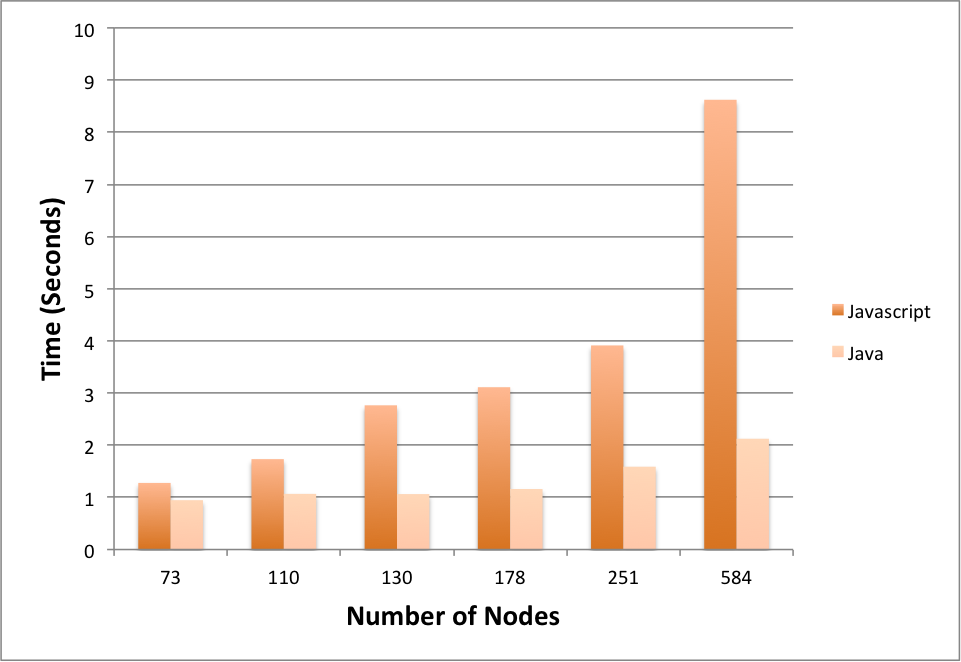
\includegraphics[width=90mm]{figures/chart.png}
\caption{\label{fig:chart}
  A chart showing the computation time required relative to the number
  of nodes in the dataset.
}
\end{figure}

As can be seen in \ref{fig:chart} the javascript implementation was
consistantly slower, as was to be expected since javascript is
typically a slower language and was being run within a
browser. However, the difference is within well within an order of
magnitude, and quite insignificant for the smaller datasets. 

Of course, our javascript implementation is also meant to be used on
websites, which are much more sensitive to latency than native
applications. Even given this, the performance on the first four
datasets is within reasonable limits for users to wait for a page to
load. 

\begin{figure}
\centering
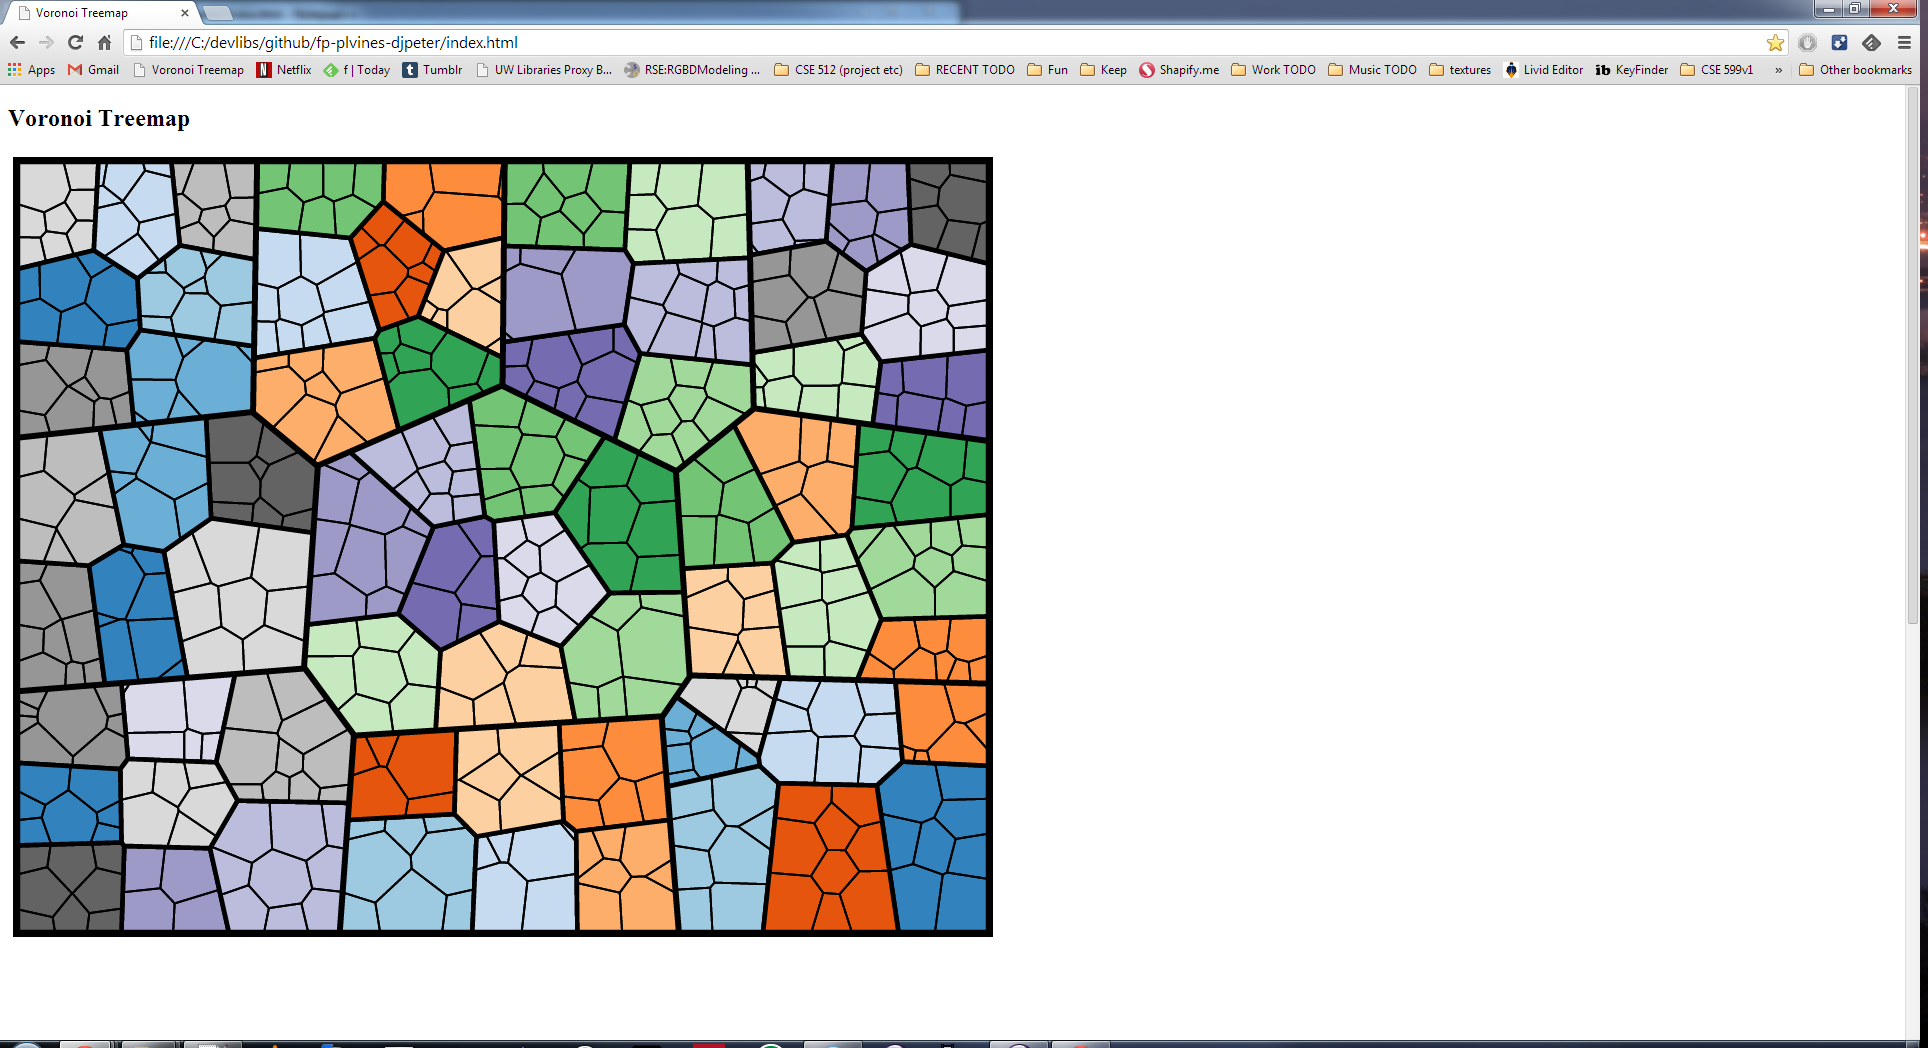
\includegraphics[width=90mm]{source images/random-10-3-025-rect.png}
\caption{}
\end{figure}
\begin{figure}
\centering
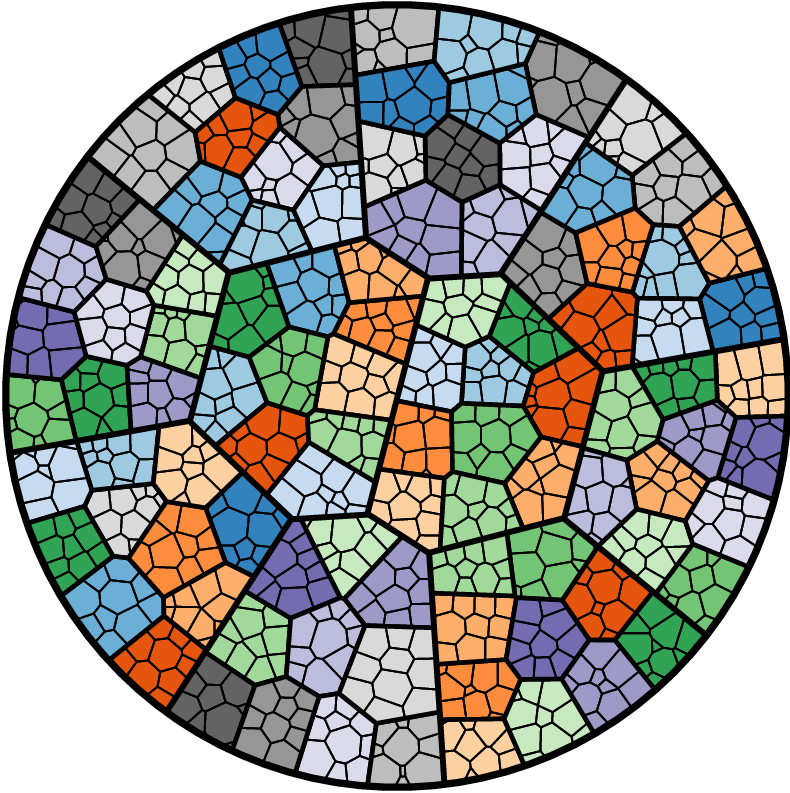
\includegraphics[width=90mm]{source images/random-10-3-000-circle.png}
\caption{}
\end{figure}
\begin{figure}
\centering
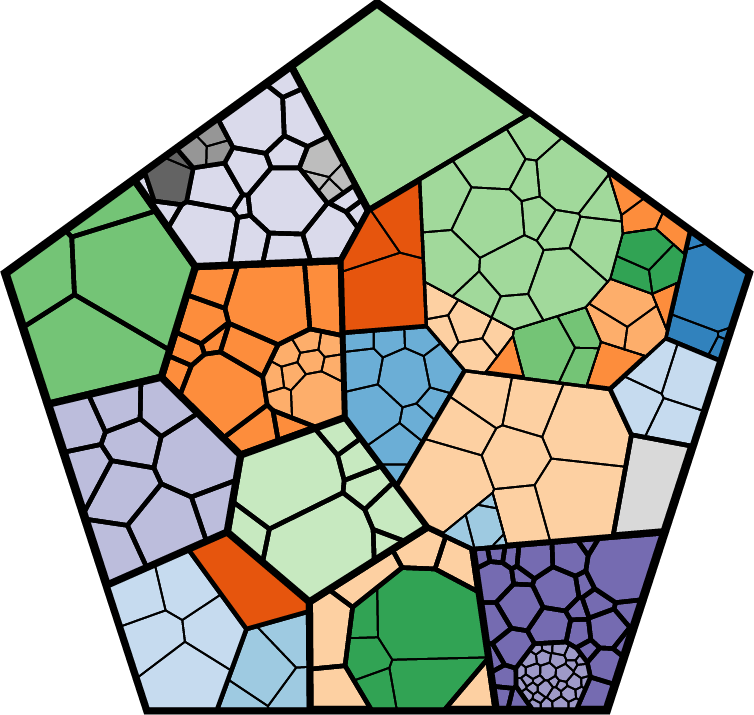
\includegraphics[width=90mm]{source images/flare-color-pentagon-100.png}
\caption{}
\end{figure}


\section{Discussion}


\section{Future Work}


\section{Acknowledgments}


\section{References}


\bibliography{writeup}{}
\bibliographystyle{plain}
\end{document}
